\documentclass[Interploate_hadwritten_Digits.tex]{subfiles}

\begin{document}
	Betrachtet man die Funktionsweise von Künstlichen Neuronalen Netzen, erkennt man eine einfache Serie von Matrixmultiplikationen und Vektoradditionen, welche einen Punkt im Problemraum in einen Punkt im Zielraum transformieren. Dies ist in der Abbildung \ref{fig:feedforward} zu sehen. Um das Netzwerk lernen zu lassen, müssen die Werte in diesen Matrizen und Vektoren so angepasst werden, dass diese die gestellte Aufgabe besser lösen. Schwierig hingegen ist das Interpretieren des Gelernten. Weshalb stehet in der ersten Gewichtsmatrix in der zweiten Zeile und fünften Spalte genau dieser Wert. Ist dieser Wert korrekt?
	\begin{Figure}
		\centering
		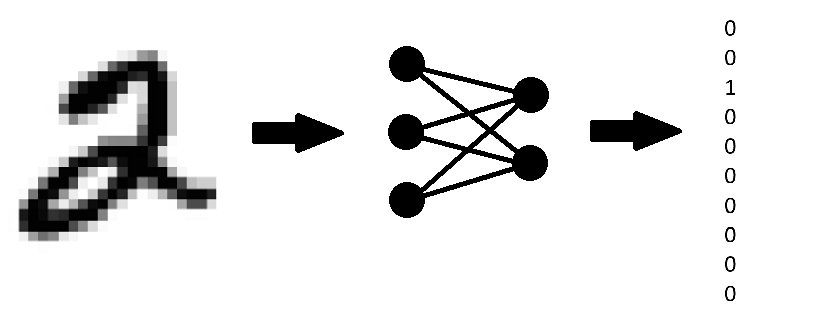
\includegraphics[width=\linewidth]{img/scribble_forward_feed.png}
		\captionof{figure}{Standard Prozess eines Neuronalen Netzes}
		\label{fig:feedforward}
	\end{Figure}
	Diese Arbeit befasst sich mit dieser Problematik und versucht gewisse ``Gedankengänge'' eines Künstlichen Neuronalen Netzes zu visualisieren. Analysiert werden die Vorgänge in einem Deep Feed-Forward Neuronal Network, welches zur Erkennung handgeschriebenen Ziffern aus dem MNIST Datensatz trainiert wurde. Für die Visualisierung wird das Inverse des Neuronalen Netzes berechnet und gezielt mit Daten gespiesen um Bilder zu produzieren. Dieser Prozess wurde in der Abbildung \ref{fig:feedbackwards} visualisiert.
	\begin{Figure}
		\centering
		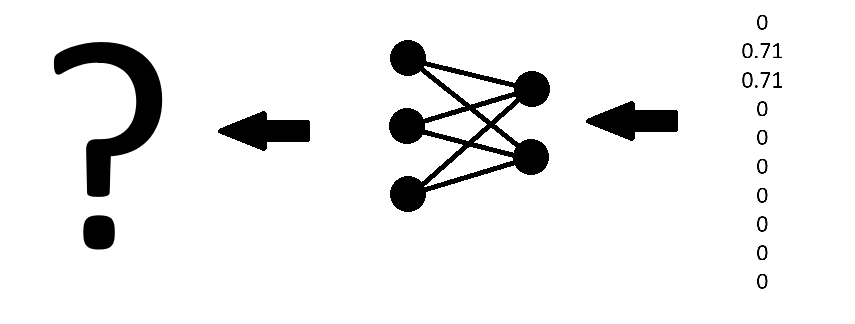
\includegraphics[width=\linewidth]{img/scribble_reverse_feed.png}
		\captionof{figure}{Intertierung des Neuronalen Netzes}
		\label{fig:feedbackwards}
	\end{Figure}
	Die Ausgabe des trainierten Neuronalen Netzes ist ein Vektor der Länge zehn. Jeder Wert in diesem Vektor gibt an, wie sicher sich das Netzwerkt ist, diese Ziffer im bewerteten Bild entdeckt zu haben. Der Index des Wertes gibt Aufschluss über die Ziffer. So wird der Index mit der höchsten Wahrscheinlichkeit als Resultat gewertet.
	
	Als Input für das invertierte Netzwerk sollen zwei verschiedene Vektortypen verwendet werden. Dies sollen einerseits ``perfekte'' Ziffervektoren sein, welche eine Eins am Index der Ziffern haben und den Rest mit Nullen besetzt ist. Andererseits sollen Vektoren von interpolierten Ziffern verwendet werden, welche eine Mischung aus zwei verschiedenen Ziffern darstellen. Diese Interpolation soll durch eine Rotation zwischen den beiden idealen Ziffervektoren realisiert werden. Dabei kann der Winkel der Rotation als Parameter für das Mischverhältnis der beiden Ziffern betrachtet werden.
	
	Somit zur Fragestellung dieser Arbeit: Lassen sich die ursprünglichen Ziffern der Interpolation nach der Rückrechnung in den Problemraum erkennen?
\end{document}